\section{Описание}

АВЛ-дерево (англ. AVL-Tree) — сбалансированное двоичное дерево поиска, в котором поддерживается следующее свойство: для каждой его вершины высота её двух поддеревьев различается не более чем на 1.


АВЛ-деревья названы по первым буквам фамилий их изобретателей, Г. М. Адельсона-Вельского и Е. М. Ландиса, которые впервые предложили использовать АВЛ-деревья в 1962 году.


АВЛ-дерево — это прежде всего двоичное дерево поиска, ключи которого удовлетворяют стандартному свойству: ключ любого узла дерева не меньше любого ключа в левом поддереве данного узла и не больше любого ключа в правом поддереве этого узла. Это значит, что для поиска нужного ключа в АВЛ-дереве можно использовать стандартный алгоритм.


Особенностью АВЛ-дерева является то, что оно является сбалансированным в следующем смысле: для любого узла дерева высота его правого поддерева отличается от высоты левого поддерева не более чем на единицу.


Традиционно, узлы АВЛ-дерева хранят не высоту, а разницу высот правого и левого поддеревьев (так называемый balance factor), которая может принимать только три значения -1, 0 и 1.


В процессе добавления или удаления узлов в АВЛ-дереве возможно возникновение ситуации, когда balance factor некоторых узлов оказывается равными 2 или -2, т.е. возникает расбалансировка поддерева. Для выправления ситуации применяются хорошо нам известные повороты вокруг тех или иных узлов дерева.


Простой поворот вправо (влево) производит следующую трансформацию дерева:


\begin{figure}[!ht]
\begin{center}
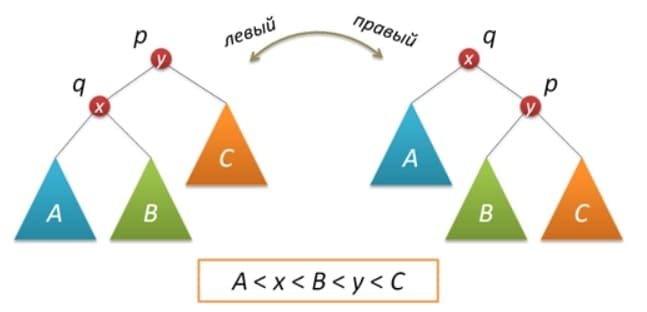
\includegraphics[scale=0.5]{./images/0.jpg}\caption{}\label{figure1}
\end{center}
\end{figure}

Рассмотрим теперь ситуацию дисбаланса, когда высота правого поддерева узла p на 2 больше высоты левого поддерева (обратный случай является симметричным и реализуется аналогично).
Пусть q — правый дочерний узел узла p, а s — левый дочерний узел узла q.

\begin{figure}[!ht]
\begin{center}
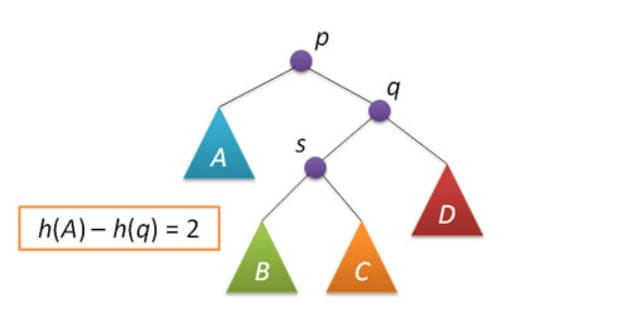
\includegraphics[scale=0.5]{./images/1.jpg}\caption{}\label{figure1}
\end{center}
\end{figure}

Анализ возможных случаев в рамках данной ситуации показывает, что для исправления расбалансировки в узле p достаточно выполнить либо простой поворот влево вокруг p, либо так называемый большой поворот влево вокруг того же p. Простой поворот выполняется при условии,
что высота левого поддерева узла q больше высоты его правого поддерева: h(s) <= h(D).

\begin{figure}[!ht]
\begin{center}
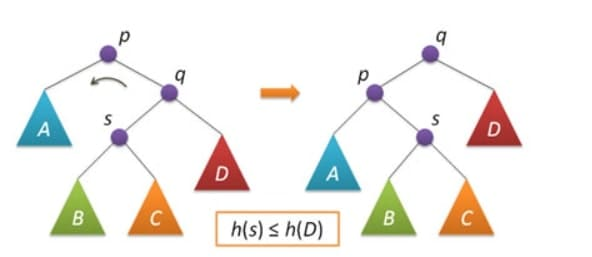
\includegraphics[scale=0.5]{./images/2.jpg}\caption{}\label{figure1}
\end{center}
\end{figure}

Большой поворот применяется при условии h(s)>h(D) и сводится в данном случае к двум простым — сначала правый поворот вокруг q и затем левый вокруг p.

\begin{figure}[!ht]
\begin{center}
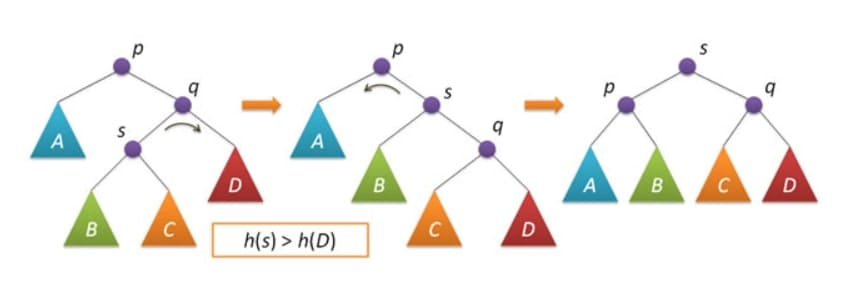
\includegraphics[scale=0.5]{./images/3.jpg}\caption{}\label{figure1}
\end{center}
\end{figure}

Вставка нового ключа в АВЛ-дерево выполняется, по большому счету, так же, как это делается в простых деревьях поиска: спускаемся вниз по дереву, выбирая правое или левое направление движения в зависимости от результата сравнения ключа в текущем узле и вставляемого ключа.
Единственное отличие заключается в том, что при возвращении из рекурсии (т.е. после того, как ключ вставлен либо в правое, либо в левое поддерево, и это дерево сбалансировано)
выполняется балансировка текущего узла.

Удаление. Идея следующая: находим узел p с заданным ключом k (если не находим, то делать ничего не надо), в правом поддереве находим узел min с наименьшим ключом и заменяем удаляемый узел p на найденный узел min. Вызываем балансировку узла.

\pagebreak

\section{Исходный код}
Cтруктура программы состоит из 2 файлов:

1. $avl.hpp$ В нем содержится объявление и реализация класса АВЛ-дерева.

2. $main\_cpp$ Обработка команд.
 
\begin{lstlisting}[language=C++]
	#ifndef AVL_H
	#define AVL_H
	
	
	#include <algorithm>
	#include <cstddef>
	#include <fstream>
	#include <iostream>
	#include <stdexcept>
	#include <string>
	#include <utility>
	
	class TAVlTree {
		private:
		struct TNode {
			std::string key;
			unsigned long long value;
			int height;
			TNode* left;
			TNode* right;
			TNode(std::string& key, unsigned long long value) {
				this->key = std::move(key);
				this->value = value;
				left = nullptr;
				right = nullptr;
				height = 1;
			}
		};
	
		TNode* root;
	
		int Height(TNode* node) // O(1) node->height
	
		int BFactor(TNode* node); // balance factor O(1) node->right->height - node->left->height
	
		void FixHeight(TNode* node); // O(1)
	
		TNode* RotateRight(TNode* node); // O(1)
	
		TNode* RotateLeft(TNode* node); // O(1)
	
		TNode* Balance(TNode* node); // O(1)
	
		TNode* Insert(TNode* node, std::string& key, unsigned long long value); O(log n)
	
		TNode* Find(TNode* node, std::string& key); // O(log n)
	
		TNode* FindMin(TNode* node); // O(log n)
	
		TNode* RemoveMin(TNode* node); // O(log n)
	
		TNode* Erase(TNode* node, std::string& key); // O(log n)
	
		void Destroy(TNode*& node); // O(n)
	
		void Destroy(); // O(n)
	
		size_t Size(TNode* node); // O(n)
	
		size_t HeightTree(TNode* node); // O(1) node->height
	
		void SaveToFile(std::ofstream& file, TNode* node); // O(n)
	
		public:
	
		TAVlTree();
	
		~TAVlTree();
	
		void Insert(std::string& key, unsigned long long value); // adding a node O(log n)

		void Erase(std::string& key); // deleting a node O(log n)
	
		std::pair<unsigned long long, bool> Exist(std::string& key); // O(log n)
	
		size_t Size(); // count of nodes O(n)
	
		void Clear(); // clear tree O(n)
	
		bool Empty(); // checking for emptiness O(1)
	
		size_t HeightTree(); // height of tree O(1)
	
		void SaveToFile(std::ofstream& file); // O(n)
	
		void LoadFromFile(std::ifstream& file); // O(n * log n)

	}
	#endif
	
\end{lstlisting}

\begin{lstlisting}[language=C++]
	#include <iostream>
	#include <string>
	#include <algorithm>
	
	#include "avl.hpp"
	
	
	int main() {
		TAVlTree avl;
		std::string command;
		while (std::cin >> command) {
			if (command == "+") {
				std::string key;
				unsigned long long value;
				std::cin >> key >> value;
				std::transform(key.begin(), key.end(), key.begin(),
							   [](unsigned char symb){ return std::tolower(symb); });
				if (avl.Exist(key).second) {
					std::cout << "Exist\n";
				} else {
					avl.Insert(key, value);
					std::cout << "OK\n";
				}
			}
			else if (command == "-") {
				std::string key;
				std::cin >> key;
				std::transform(key.begin(), key.end(), key.begin(),
							   [](unsigned char symb){ return std::tolower(symb); });
				if (!avl.Exist(key).second) {
					std::cout << "NoSuchWord\n";
				} else {
					avl.Erase(key);
					std::cout << "OK\n";
				}
			
			} else if (command == "!") {
				std::string action;
				std::cin >> action;
				std::string path;
				std::cin >> path;
				if (action == "Save") {   
					std::ofstream file(path, std::ios::binary | std::ios::trunc);
					auto size = avl.Size();
					file.write(reinterpret_cast<char*>(&size), sizeof(unsigned long long));
					if (size > 0) {
						avl.SaveToFile(file);
					}
					std::cout << "OK\n";
					file.close();
	
				} else {
					std::ifstream file(path, std::ios::binary);
					avl.LoadFromFile(file);
					std::cout << "OK\n";
					file.close();
	   
				}
	
			} else {
				std::transform(command.begin(), command.end(), command.begin(),
							   [](unsigned char symb){ return std::tolower(symb); });
				auto node = avl.Exist(command);
				if (node.second) {
					std::cout << "OK: " << node.first << "\n";
				} else {
					std::cout << "NoSuchWord\n";
				}
			}
		}
	}
\end{lstlisting}

\pagebreak

\section{Консоль}
\begin{alltt}
[alex@fedora mai-da-labs]$ cd build
[alex@fedora build]$ cmake ../
-- Configuring done (0.3s)
-- Generating done (0.0s)
-- Build files have been written to: /home/alex/mai-da-labs/build
[alex@fedora build]$ cmake --build .
[2/2] Linking CXX executable lab2_avl/lab2_avl
[alex@fedora build]$ cd lab2_avl
[alex@fedora lab2_avl]$ ls
CMakeFiles  cmake_install.cmake  CTestTestfile.cmake  lab2_avl  test.txt
[alex@fedora lab2_avl]$ cat test.txt 
+ a 1
+ A 2
+ aaaaaaaaaaaaaaaaaaaaaaaaaaaaaaaaaaaaaaaaaaaaaaaaaaaaaaaaaaaaaaaaaaaaaaaaaaaaaaaaaaaaaaaaaaaaaaaaaaaaaaaaaaaaaaaaaaaaaaaaaaaaaaaaaaaaaaaaaaaaaaaaaaaaaaaaaaaaaaaaaaaaaaaaaaaaaaaaaaaaaaaaaaaaaaaaaaaaaaaaaaaaaaaaaaaaaaaaaaaaaaaaaaaaaaaaaaaaaaaaaaaaaaaaaaaaaaaa 18446744073709551615
aaaaaaaaaaaaaaaaaaaaaaaaaaaaaaaaaaaaaaaaaaaaaaaaaaaaaaaaaaaaaaaaaaaaaaaaaaaaaaaaaaaaaaaaaaaaaaaaaaaaaaaaaaaaaaaaaaaaaaaaaaaaaaaaaaaaaaaaaaaaaaaaaaaaaaaaaaaaaaaaaaaaaaaaaaaaaaaaaaaaaaaaaaaaaaaaaaaaaaaaaaaaaaaaaaaaaaaaaaaaaaaaaaaaaaaaaaaaaaaaaaaaaaaaaaaaaaaa
A
- A
a
[alex@fedora lab2_avl]$ ./lab2_avl <test.txt 
OK
Exist
OK
OK: 18446744073709551615
OK: 1
OK
NoSuchWord	
\end{alltt}
\pagebreak

